\exer{[polynome]}
\setcounter{numques}{0}~\\

\question{} Poser le système d'équations à résoudre.

\begin{align*}
\left\{
\begin{array}{l}
a\times(-1)^2+b\times (-1)+c=9\\
\\
a\times(1)^2+b\times (1)+c=3\\
\\
a\times(2)^2+b\times (2)+c=3\\
\end{array}
\right.
\end{align*}

\question{} Déterminer les coefficients $a$, $b$ et $c$ par l'utilisation du pivot de Gauss.

\begin{lstlisting}
A=array([[(-1.)**2,-1.,1.],[1.**2,1.,1.],[2.**2,2.,1.]])
b=array([[9.],[3.],[3.]])

X=resout(A,b)
\end{lstlisting}

\question{} Sur un même graphe faire apparaître les 3 points ainsi que la paraboles obtenue par interpolation.
\begin{lstlisting}
def f(x):
    return X[0]*x**2+X[1]*x+X[2]

vx=np.linspace(-3,3,101)
plt.plot([-1,1,2],[9,3,3],'b*')
plt.plot(vx,f(vx),'r-',label='$y=a\cdot x^2+b\cdot x+c$')
plt.xlabel('x')
plt.ylabel('y')
plt.legend()
plt.savefig('tp_13_q03_durif.png')
\end{lstlisting}

\begin{center}
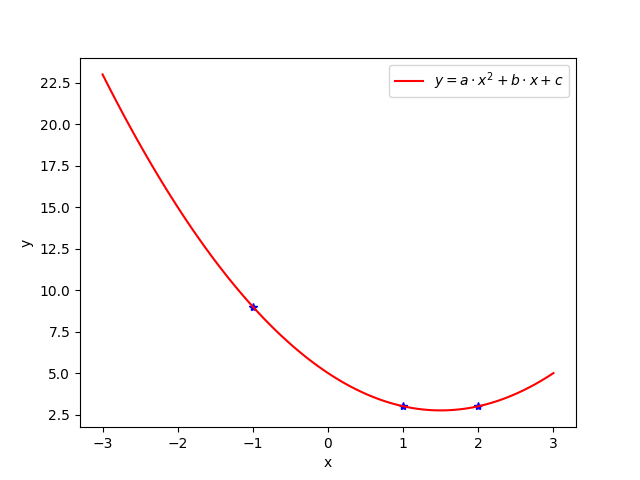
\includegraphics[width=0.5\textwidth]{polynome.png}
\end{center}